% Options for packages loaded elsewhere
\PassOptionsToPackage{unicode}{hyperref}
\PassOptionsToPackage{hyphens}{url}
%
\documentclass[
]{article}
\usepackage{amsmath,amssymb}
\usepackage{iftex}
\ifPDFTeX
  \usepackage[T1]{fontenc}
  \usepackage[utf8]{inputenc}
  \usepackage{textcomp} % provide euro and other symbols
\else % if luatex or xetex
  \usepackage{unicode-math} % this also loads fontspec
  \defaultfontfeatures{Scale=MatchLowercase}
  \defaultfontfeatures[\rmfamily]{Ligatures=TeX,Scale=1}
\fi
\usepackage{lmodern}
\ifPDFTeX\else
  % xetex/luatex font selection
\fi
% Use upquote if available, for straight quotes in verbatim environments
\IfFileExists{upquote.sty}{\usepackage{upquote}}{}
\IfFileExists{microtype.sty}{% use microtype if available
  \usepackage[]{microtype}
  \UseMicrotypeSet[protrusion]{basicmath} % disable protrusion for tt fonts
}{}
\makeatletter
\@ifundefined{KOMAClassName}{% if non-KOMA class
  \IfFileExists{parskip.sty}{%
    \usepackage{parskip}
  }{% else
    \setlength{\parindent}{0pt}
    \setlength{\parskip}{6pt plus 2pt minus 1pt}}
}{% if KOMA class
  \KOMAoptions{parskip=half}}
\makeatother
\usepackage{xcolor}
\usepackage[margin=1in]{geometry}
\usepackage{color}
\usepackage{fancyvrb}
\newcommand{\VerbBar}{|}
\newcommand{\VERB}{\Verb[commandchars=\\\{\}]}
\DefineVerbatimEnvironment{Highlighting}{Verbatim}{commandchars=\\\{\}}
% Add ',fontsize=\small' for more characters per line
\usepackage{framed}
\definecolor{shadecolor}{RGB}{248,248,248}
\newenvironment{Shaded}{\begin{snugshade}}{\end{snugshade}}
\newcommand{\AlertTok}[1]{\textcolor[rgb]{0.94,0.16,0.16}{#1}}
\newcommand{\AnnotationTok}[1]{\textcolor[rgb]{0.56,0.35,0.01}{\textbf{\textit{#1}}}}
\newcommand{\AttributeTok}[1]{\textcolor[rgb]{0.13,0.29,0.53}{#1}}
\newcommand{\BaseNTok}[1]{\textcolor[rgb]{0.00,0.00,0.81}{#1}}
\newcommand{\BuiltInTok}[1]{#1}
\newcommand{\CharTok}[1]{\textcolor[rgb]{0.31,0.60,0.02}{#1}}
\newcommand{\CommentTok}[1]{\textcolor[rgb]{0.56,0.35,0.01}{\textit{#1}}}
\newcommand{\CommentVarTok}[1]{\textcolor[rgb]{0.56,0.35,0.01}{\textbf{\textit{#1}}}}
\newcommand{\ConstantTok}[1]{\textcolor[rgb]{0.56,0.35,0.01}{#1}}
\newcommand{\ControlFlowTok}[1]{\textcolor[rgb]{0.13,0.29,0.53}{\textbf{#1}}}
\newcommand{\DataTypeTok}[1]{\textcolor[rgb]{0.13,0.29,0.53}{#1}}
\newcommand{\DecValTok}[1]{\textcolor[rgb]{0.00,0.00,0.81}{#1}}
\newcommand{\DocumentationTok}[1]{\textcolor[rgb]{0.56,0.35,0.01}{\textbf{\textit{#1}}}}
\newcommand{\ErrorTok}[1]{\textcolor[rgb]{0.64,0.00,0.00}{\textbf{#1}}}
\newcommand{\ExtensionTok}[1]{#1}
\newcommand{\FloatTok}[1]{\textcolor[rgb]{0.00,0.00,0.81}{#1}}
\newcommand{\FunctionTok}[1]{\textcolor[rgb]{0.13,0.29,0.53}{\textbf{#1}}}
\newcommand{\ImportTok}[1]{#1}
\newcommand{\InformationTok}[1]{\textcolor[rgb]{0.56,0.35,0.01}{\textbf{\textit{#1}}}}
\newcommand{\KeywordTok}[1]{\textcolor[rgb]{0.13,0.29,0.53}{\textbf{#1}}}
\newcommand{\NormalTok}[1]{#1}
\newcommand{\OperatorTok}[1]{\textcolor[rgb]{0.81,0.36,0.00}{\textbf{#1}}}
\newcommand{\OtherTok}[1]{\textcolor[rgb]{0.56,0.35,0.01}{#1}}
\newcommand{\PreprocessorTok}[1]{\textcolor[rgb]{0.56,0.35,0.01}{\textit{#1}}}
\newcommand{\RegionMarkerTok}[1]{#1}
\newcommand{\SpecialCharTok}[1]{\textcolor[rgb]{0.81,0.36,0.00}{\textbf{#1}}}
\newcommand{\SpecialStringTok}[1]{\textcolor[rgb]{0.31,0.60,0.02}{#1}}
\newcommand{\StringTok}[1]{\textcolor[rgb]{0.31,0.60,0.02}{#1}}
\newcommand{\VariableTok}[1]{\textcolor[rgb]{0.00,0.00,0.00}{#1}}
\newcommand{\VerbatimStringTok}[1]{\textcolor[rgb]{0.31,0.60,0.02}{#1}}
\newcommand{\WarningTok}[1]{\textcolor[rgb]{0.56,0.35,0.01}{\textbf{\textit{#1}}}}
\usepackage{graphicx}
\makeatletter
\def\maxwidth{\ifdim\Gin@nat@width>\linewidth\linewidth\else\Gin@nat@width\fi}
\def\maxheight{\ifdim\Gin@nat@height>\textheight\textheight\else\Gin@nat@height\fi}
\makeatother
% Scale images if necessary, so that they will not overflow the page
% margins by default, and it is still possible to overwrite the defaults
% using explicit options in \includegraphics[width, height, ...]{}
\setkeys{Gin}{width=\maxwidth,height=\maxheight,keepaspectratio}
% Set default figure placement to htbp
\makeatletter
\def\fps@figure{htbp}
\makeatother
\setlength{\emergencystretch}{3em} % prevent overfull lines
\providecommand{\tightlist}{%
  \setlength{\itemsep}{0pt}\setlength{\parskip}{0pt}}
\setcounter{secnumdepth}{-\maxdimen} % remove section numbering
\usepackage{booktabs}
\usepackage{longtable}
\usepackage{array}
\usepackage{multirow}
\usepackage{wrapfig}
\usepackage{float}
\usepackage{colortbl}
\usepackage{pdflscape}
\usepackage{tabu}
\usepackage{threeparttable}
\usepackage{threeparttablex}
\usepackage[normalem]{ulem}
\usepackage{makecell}
\usepackage{xcolor}
\ifLuaTeX
  \usepackage{selnolig}  % disable illegal ligatures
\fi
\usepackage{bookmark}
\IfFileExists{xurl.sty}{\usepackage{xurl}}{} % add URL line breaks if available
\urlstyle{same}
\hypersetup{
  pdftitle={Software code},
  pdfauthor={Wiem Ben Romdhane},
  hidelinks,
  pdfcreator={LaTeX via pandoc}}

\title{Software code}
\author{Wiem Ben Romdhane}
\date{2025-03-26}

\begin{document}
\maketitle

\section{Import libraries}\label{import-libraries}

\begin{Shaded}
\begin{Highlighting}[]
\ImportTok{import}\NormalTok{ pandas }\ImportTok{as}\NormalTok{ pd}
\ImportTok{import}\NormalTok{ numpy }\ImportTok{as}\NormalTok{ np}
\ImportTok{import}\NormalTok{ matplotlib.pyplot }\ImportTok{as}\NormalTok{ plt}
\ImportTok{import}\NormalTok{ keras\_tuner }\ImportTok{as}\NormalTok{ kt}
\ImportTok{from}\NormalTok{ tensorflow.keras.models }\ImportTok{import}\NormalTok{ Sequential}
\ImportTok{from}\NormalTok{ tensorflow.keras.layers }\ImportTok{import}\NormalTok{ LSTM, GRU, Dense, Dropout}
\ImportTok{from}\NormalTok{ tensorflow.keras.optimizers }\ImportTok{import}\NormalTok{ Adam}
\ImportTok{from}\NormalTok{ tensorflow.keras.callbacks }\ImportTok{import}\NormalTok{ EarlyStopping}
\ImportTok{from}\NormalTok{ sklearn.model\_selection }\ImportTok{import}\NormalTok{ train\_test\_split}
\ImportTok{from}\NormalTok{ sklearn.preprocessing }\ImportTok{import}\NormalTok{ MinMaxScaler}
\end{Highlighting}
\end{Shaded}

\section{Import data}\label{import-data}

\begin{Shaded}
\begin{Highlighting}[]
\NormalTok{url}\OperatorTok{=}\StringTok{"https://raw.githubusercontent.com/Hamrita/Wiem\_paper01/refs/heads/main/Data/crypto.csv"}
\NormalTok{crypto}\OperatorTok{=}\NormalTok{pd.read\_csv(url)}
\NormalTok{BTC}\OperatorTok{=}\NormalTok{df.iloc[:,}\DecValTok{1}\NormalTok{].values.astype(}\StringTok{\textquotesingle{}float32\textquotesingle{}}\NormalTok{)}
\NormalTok{BTC}\OperatorTok{=}\NormalTok{BTC.reshape(BTC.shape[}\DecValTok{0}\NormalTok{],}\DecValTok{1}\NormalTok{)}
\NormalTok{ETH}\OperatorTok{=}\NormalTok{df.iloc[:,}\DecValTok{2}\NormalTok{].values.astype(}\StringTok{\textquotesingle{}float32\textquotesingle{}}\NormalTok{)}
\NormalTok{ETH}\OperatorTok{=}\NormalTok{ETH.reshape(ETH.shape[}\DecValTok{0}\NormalTok{],}\DecValTok{1}\NormalTok{)}
\NormalTok{LTC}\OperatorTok{=}\NormalTok{df.iloc[:,}\DecValTok{3}\NormalTok{].values.astype(}\StringTok{\textquotesingle{}float32\textquotesingle{}}\NormalTok{)}
\NormalTok{LTC}\OperatorTok{=}\NormalTok{LTC.reshape(LTC.shape[}\DecValTok{0}\NormalTok{],}\DecValTok{1}\NormalTok{)}
\end{Highlighting}
\end{Shaded}

\section{Split data}\label{split-data}

\begin{Shaded}
\begin{Highlighting}[]
\CommentTok{\# Split into train and test sets}
\NormalTok{nn}\OperatorTok{=}\BuiltInTok{len}\NormalTok{(BTC)}
\NormalTok{train\_size }\OperatorTok{=} \BuiltInTok{int}\NormalTok{(nn }\OperatorTok{*} \FloatTok{0.9}\NormalTok{)}
\NormalTok{test\_size }\OperatorTok{=}\NormalTok{ nn }\OperatorTok{{-}}\NormalTok{ train\_size}
\NormalTok{trainBTC, testBTC }\OperatorTok{=}\NormalTok{ BTC[}\DecValTok{0}\NormalTok{:train\_size], BTC[train\_size:nn]}
\NormalTok{trainETH, testETH }\OperatorTok{=}\NormalTok{ ETH[}\DecValTok{0}\NormalTok{:train\_size], ETH[train\_size:nn]}
\NormalTok{trainLTC, testLTC }\OperatorTok{=}\NormalTok{ LTC[}\DecValTok{0}\NormalTok{:train\_size], LTC[train\_size:nn]}
\end{Highlighting}
\end{Shaded}

\section{Scale data}\label{scale-data}

\begin{Shaded}
\begin{Highlighting}[]
\NormalTok{scalerBTC }\OperatorTok{=}\NormalTok{ MinMaxScaler(feature\_range}\OperatorTok{=}\NormalTok{(}\DecValTok{0}\NormalTok{, }\DecValTok{1}\NormalTok{))}
\NormalTok{trainBTC\_scaled }\OperatorTok{=}\NormalTok{ scalerBTC.fit\_transform(trainBTC)}
\NormalTok{testBTC\_scaled}\OperatorTok{=}\NormalTok{scalerBTC.transform(testBTC)}
\NormalTok{scalerETH }\OperatorTok{=}\NormalTok{ MinMaxScaler(feature\_range}\OperatorTok{=}\NormalTok{(}\DecValTok{0}\NormalTok{, }\DecValTok{1}\NormalTok{))}
\NormalTok{trainETH\_scaled }\OperatorTok{=}\NormalTok{ scalerETH.fit\_transform(trainETH)}
\NormalTok{testETH\_scaled}\OperatorTok{=}\NormalTok{scalerETH.transform(testETH)}
\NormalTok{scalerLTC }\OperatorTok{=}\NormalTok{ MinMaxScaler(feature\_range}\OperatorTok{=}\NormalTok{(}\DecValTok{0}\NormalTok{, }\DecValTok{1}\NormalTok{))}
\NormalTok{trainLTC\_scaled }\OperatorTok{=}\NormalTok{ scalerLTC.fit\_transform(trainLTC)}
\NormalTok{testLTC\_scaled}\OperatorTok{=}\NormalTok{scalerLTC.transform(testLTC)}
\end{Highlighting}
\end{Shaded}

\section{Create sequences}\label{create-sequences}

\begin{Shaded}
\begin{Highlighting}[]
\KeywordTok{def}\NormalTok{ create\_dataset(dataset, look\_back}\OperatorTok{=}\DecValTok{1}\NormalTok{):}
\NormalTok{    dataX, dataY }\OperatorTok{=}\NormalTok{ [], []}
    \ControlFlowTok{for}\NormalTok{ i }\KeywordTok{in} \BuiltInTok{range}\NormalTok{(}\BuiltInTok{len}\NormalTok{(dataset)}\OperatorTok{{-}}\NormalTok{look\_back}\OperatorTok{{-}}\DecValTok{1}\NormalTok{):}
\NormalTok{        a }\OperatorTok{=}\NormalTok{ dataset[i:(i}\OperatorTok{+}\NormalTok{look\_back), :]  }\CommentTok{\#get look\_back sequences}
\NormalTok{        dataX.append(a)}
\NormalTok{        dataY.append(dataset[i }\OperatorTok{+}\NormalTok{ look\_back, }\DecValTok{0}\NormalTok{]) }\CommentTok{\#get the target after look\_back sequences}
    \ControlFlowTok{return}\NormalTok{ np.array(dataX), np.array(dataY)}
\end{Highlighting}
\end{Shaded}

\begin{Shaded}
\begin{Highlighting}[]
\NormalTok{look\_back }\OperatorTok{=} \DecValTok{10}  \CommentTok{\# Sequence length (tunable)}
\NormalTok{trainX\_BTC, trainY\_BTC }\OperatorTok{=}\NormalTok{ create\_dataset(trainBTC\_scaled, look\_back)}
\NormalTok{testX\_BTC, testY\_BTC }\OperatorTok{=}\NormalTok{ create\_dataset(testBTC\_scaled, look\_back)}

\NormalTok{trainX\_ETH, trainY\_ETH }\OperatorTok{=}\NormalTok{ create\_dataset(trainETH\_scaled, look\_back)}
\NormalTok{testX\_ETH, testY\_ETH }\OperatorTok{=}\NormalTok{ create\_dataset(testETH\_scaled, look\_back)}

\NormalTok{trainX\_LTC, trainY\_LTC }\OperatorTok{=}\NormalTok{ create\_dataset(trainLTC\_scaled, look\_back)}
\NormalTok{testX\_LTC, testY\_LTC }\OperatorTok{=}\NormalTok{ create\_dataset(testLTC\_scaled, look\_back)}
\end{Highlighting}
\end{Shaded}

\begin{Shaded}
\begin{Highlighting}[]
\KeywordTok{def}\NormalTok{ build\_model1(hp):}
\NormalTok{    model }\OperatorTok{=}\NormalTok{ Sequential()}
\NormalTok{    model.add(LSTM(hp.Int(}\StringTok{\textquotesingle{}input\_unit\textquotesingle{}}\NormalTok{,min\_value}\OperatorTok{=}\DecValTok{50}\NormalTok{,max\_value}\OperatorTok{=}\DecValTok{200}\NormalTok{, step}\OperatorTok{=}\DecValTok{50}\NormalTok{),return\_sequences}\OperatorTok{=}\VariableTok{True}\NormalTok{, input\_shape}\OperatorTok{=}\NormalTok{(trainX\_BTC.shape[}\DecValTok{1}\NormalTok{],trainX\_BTC.shape[}\DecValTok{2}\NormalTok{])))}
    \ControlFlowTok{for}\NormalTok{ i }\KeywordTok{in} \BuiltInTok{range}\NormalTok{(hp.Int(}\StringTok{\textquotesingle{}n\_layers\textquotesingle{}}\NormalTok{, }\DecValTok{1}\NormalTok{, }\DecValTok{3}\NormalTok{)):}
\NormalTok{        model.add(LSTM(hp.Int(}\SpecialStringTok{f\textquotesingle{}lstm\_}\SpecialCharTok{\{}\NormalTok{i}\SpecialCharTok{\}}\SpecialStringTok{\_units\textquotesingle{}}\NormalTok{,min\_value}\OperatorTok{=}\DecValTok{50}\NormalTok{,max\_value}\OperatorTok{=}\DecValTok{200}\NormalTok{, step}\OperatorTok{=}\DecValTok{50}\NormalTok{),return\_sequences}\OperatorTok{=}\VariableTok{True}\NormalTok{))}
\NormalTok{    model.add(LSTM(hp.Int(}\StringTok{\textquotesingle{}layer\_2\_neurons\textquotesingle{}}\NormalTok{,min\_value}\OperatorTok{=}\DecValTok{50}\NormalTok{,max\_value}\OperatorTok{=}\DecValTok{200}\NormalTok{, step}\OperatorTok{=}\DecValTok{50}\NormalTok{)))}
\NormalTok{    model.add(Dropout(hp.Float(}\StringTok{\textquotesingle{}Dropout\_rate\textquotesingle{}}\NormalTok{,min\_value}\OperatorTok{=}\FloatTok{0.1}\NormalTok{,max\_value}\OperatorTok{=}\FloatTok{0.6}\NormalTok{,step}\OperatorTok{=}\FloatTok{0.1}\NormalTok{)))}
\NormalTok{    model.add(Dense(}\DecValTok{1}\NormalTok{, activation}\OperatorTok{=}\NormalTok{hp.Choice(}\StringTok{\textquotesingle{}dense\_activation\textquotesingle{}}\NormalTok{,values}\OperatorTok{=}\NormalTok{[}\StringTok{\textquotesingle{}relu\textquotesingle{}}\NormalTok{, }\StringTok{\textquotesingle{}sigmoid\textquotesingle{}}\NormalTok{],default}\OperatorTok{=}\StringTok{\textquotesingle{}relu\textquotesingle{}}\NormalTok{)))}
\NormalTok{    learning\_rate }\OperatorTok{=}\NormalTok{ hp.Float(}\StringTok{\textquotesingle{}learning\_rate\textquotesingle{}}\NormalTok{, min\_value}\OperatorTok{=}\FloatTok{1e{-}4}\NormalTok{, max\_value}\OperatorTok{=}\FloatTok{1e{-}2}\NormalTok{, sampling}\OperatorTok{=}\StringTok{\textquotesingle{}log\textquotesingle{}}\NormalTok{)}
\NormalTok{    model.}\BuiltInTok{compile}\NormalTok{(loss}\OperatorTok{=}\StringTok{\textquotesingle{}mean\_squared\_error\textquotesingle{}}\NormalTok{, optimizer}\OperatorTok{=}\NormalTok{Adam(learning\_rate}\OperatorTok{=}\NormalTok{learning\_rate),metrics }\OperatorTok{=}\NormalTok{ [}\StringTok{\textquotesingle{}mae\textquotesingle{}}\NormalTok{])}
    \ControlFlowTok{return}\NormalTok{ model}
\end{Highlighting}
\end{Shaded}

\begin{Shaded}
\begin{Highlighting}[]
\NormalTok{tuner1}\OperatorTok{=}\NormalTok{ kt.RandomSearch(}
\NormalTok{        build\_model1,}
\NormalTok{        objective}\OperatorTok{=}\StringTok{\textquotesingle{}loss\textquotesingle{}}\NormalTok{,}
\NormalTok{        max\_trials}\OperatorTok{=}\DecValTok{10}\NormalTok{,}
\NormalTok{        executions\_per\_trial}\OperatorTok{=}\DecValTok{1}\NormalTok{,}
\NormalTok{        overwrite}\OperatorTok{=}\VariableTok{True}
\NormalTok{        )}

\CommentTok{\# Early stopping callback}
\NormalTok{early\_stopper }\OperatorTok{=}\NormalTok{ EarlyStopping(}
\NormalTok{    monitor}\OperatorTok{=}\StringTok{\textquotesingle{}loss\textquotesingle{}}\NormalTok{,}
\NormalTok{    min\_delta}\OperatorTok{=}\FloatTok{0.01}\NormalTok{,}
\NormalTok{    patience}\OperatorTok{=}\DecValTok{5}\NormalTok{,}
\NormalTok{    restore\_best\_weights}\OperatorTok{=}\VariableTok{True}
\NormalTok{)}
\end{Highlighting}
\end{Shaded}

\begin{Shaded}
\begin{Highlighting}[]
\NormalTok{tuner1.search(}
\NormalTok{        x}\OperatorTok{=}\NormalTok{trainX\_BTC,}
\NormalTok{        y}\OperatorTok{=}\NormalTok{trainY\_BTC,}
\NormalTok{        epochs}\OperatorTok{=}\DecValTok{100}\NormalTok{,}
\NormalTok{        batch\_size}\OperatorTok{=}\DecValTok{32}\NormalTok{,}
\NormalTok{        validation\_data}\OperatorTok{=}\NormalTok{(testX\_BTC,testY\_BTC),}
\NormalTok{        callbacks}\OperatorTok{=}\NormalTok{[early\_stopper]}
\NormalTok{)}
\end{Highlighting}
\end{Shaded}

\begin{Shaded}
\begin{Highlighting}[]
\NormalTok{best\_model\_btc }\OperatorTok{=}\NormalTok{ tuner1.get\_best\_models(num\_models}\OperatorTok{=}\DecValTok{1}\NormalTok{)[}\DecValTok{0}\NormalTok{]}
\end{Highlighting}
\end{Shaded}

\begin{Shaded}
\begin{Highlighting}[]
\NormalTok{best\_hyperparameters\_btc }\OperatorTok{=}\NormalTok{ tuner1.get\_best\_hyperparameters(num\_trials}\OperatorTok{=}\DecValTok{1}\NormalTok{)[}\DecValTok{0}\NormalTok{]}
\NormalTok{best\_hyperparameters\_btc.values}
\end{Highlighting}
\end{Shaded}

\begin{Shaded}
\begin{Highlighting}[]
\NormalTok{fit\_model\_btc}\OperatorTok{=}\NormalTok{best\_model\_btc.fit(trainX\_BTC,trainY\_BTC,}
\NormalTok{                            epochs}\OperatorTok{=}\DecValTok{200}\NormalTok{, verbose}\OperatorTok{=}\DecValTok{0}\NormalTok{ )}
\end{Highlighting}
\end{Shaded}

\begin{Shaded}
\begin{Highlighting}[]
\NormalTok{fit\_btc}\OperatorTok{=}\NormalTok{best\_model\_btc.predict(trainX\_BTC)}
\NormalTok{for\_btc}\OperatorTok{=}\NormalTok{best\_model\_btc.predict(testX\_BTC)}
\NormalTok{btc\_fit}\OperatorTok{=}\NormalTok{scalerBTC.inverse\_transform(fit\_btc)}
\NormalTok{btc\_pred}\OperatorTok{=}\NormalTok{scalerBTC.inverse\_transform(for\_btc)}

\NormalTok{btc\_tr}\OperatorTok{=}\NormalTok{scalerBTC.inverse\_transform(trainY\_BTC.reshape(}\OperatorTok{{-}}\DecValTok{1}\NormalTok{,}\DecValTok{1}\NormalTok{))}
\NormalTok{btc\_te}\OperatorTok{=}\NormalTok{scalerBTC.inverse\_transform(testY\_BTC.reshape(}\OperatorTok{{-}}\DecValTok{1}\NormalTok{,}\DecValTok{1}\NormalTok{))}
\end{Highlighting}
\end{Shaded}

\begin{Shaded}
\begin{Highlighting}[]
\NormalTok{btc\_fit\_lstm}\OperatorTok{=}\NormalTok{pd.DataFrame(btc\_fit)}
\NormalTok{btc\_pred\_lstm}\OperatorTok{=}\NormalTok{pd.DataFrame(btc\_pred)}
\NormalTok{btc\_fit\_lstm.to\_csv(}\StringTok{\textquotesingle{}Data/btc\_fit\_lstm.csv\textquotesingle{}}\NormalTok{, index}\OperatorTok{=}\VariableTok{False}\NormalTok{)}
\NormalTok{btc\_pred\_lstm.to\_csv(}\StringTok{\textquotesingle{}Data/btc\_pred\_lstm.csv\textquotesingle{}}\NormalTok{, index}\OperatorTok{=}\VariableTok{False}\NormalTok{)}
\NormalTok{btc\_tr\_lstm}\OperatorTok{=}\NormalTok{pd.DataFrame(btc\_tr)}
\NormalTok{btc\_te\_lstm}\OperatorTok{=}\NormalTok{pd.DataFrame(btc\_te)}
\NormalTok{btc\_tr\_lstm.to\_csv(}\StringTok{\textquotesingle{}Data/btc\_tr\_lstm.csv\textquotesingle{}}\NormalTok{, index}\OperatorTok{=}\VariableTok{False}\NormalTok{)}
\NormalTok{btc\_te\_lstm.to\_csv(}\StringTok{\textquotesingle{}Data/btc\_te\_lstm.csv\textquotesingle{}}\NormalTok{, index}\OperatorTok{=}\VariableTok{False}\NormalTok{)}
\end{Highlighting}
\end{Shaded}

\begin{Shaded}
\begin{Highlighting}[]
\NormalTok{plt.plot(btc\_te,label}\OperatorTok{=}\StringTok{\textquotesingle{}Actual (Test)\textquotesingle{}}\NormalTok{)}
\NormalTok{plt.plot(btc\_pred,linestyle}\OperatorTok{=}\StringTok{"dashed"}\NormalTok{,label}\OperatorTok{=}\StringTok{\textquotesingle{}Predicted (Test)\textquotesingle{}}\NormalTok{)}
\NormalTok{plt.legend()}
\NormalTok{plt.show()}
\end{Highlighting}
\end{Shaded}

\begin{Shaded}
\begin{Highlighting}[]
\NormalTok{lstm100}\OperatorTok{=}\NormalTok{Sequential()}
\NormalTok{lstm100.add(LSTM(units}\OperatorTok{=}\DecValTok{100}\NormalTok{, return\_sequences}\OperatorTok{=}\VariableTok{True}\NormalTok{, input\_shape}\OperatorTok{=}\NormalTok{(trainX\_BTC.shape[}\DecValTok{1}\NormalTok{], }\DecValTok{1}\NormalTok{)))}
\NormalTok{lstm100.add(LSTM(units}\OperatorTok{=}\DecValTok{100}\NormalTok{, return\_sequences}\OperatorTok{=}\VariableTok{True}\NormalTok{))}
\NormalTok{lstm100.add(LSTM(units}\OperatorTok{=}\DecValTok{100}\NormalTok{))}
\NormalTok{lstm100.add(Dense(units}\OperatorTok{=}\DecValTok{1}\NormalTok{))}
\NormalTok{lstm100.}\BuiltInTok{compile}\NormalTok{(optimizer}\OperatorTok{=}\StringTok{\textquotesingle{}adam\textquotesingle{}}\NormalTok{, loss}\OperatorTok{=}\StringTok{\textquotesingle{}mean\_squared\_error\textquotesingle{}}\NormalTok{)}
\NormalTok{his\_100}\OperatorTok{=}\NormalTok{lstm100.fit(trainX\_BTC, trainY\_BTC, epochs}\OperatorTok{=}\DecValTok{100}\NormalTok{, batch\_size}\OperatorTok{=}\DecValTok{32}\NormalTok{, }
\NormalTok{           validation\_data}\OperatorTok{=}\NormalTok{(testX\_BTC, testY\_BTC))}
\end{Highlighting}
\end{Shaded}

\begin{Shaded}
\begin{Highlighting}[]
\NormalTok{fit\_btc100}\OperatorTok{=}\NormalTok{lstm100.predict(trainX\_BTC)}
\NormalTok{for\_btc100}\OperatorTok{=}\NormalTok{lstm100.predict(testX\_BTC)}
\NormalTok{btc\_fit100}\OperatorTok{=}\NormalTok{scalerBTC.inverse\_transform(fit\_btc100)}
\NormalTok{btc\_pred100}\OperatorTok{=}\NormalTok{scalerBTC.inverse\_transform(for\_btc100)}

\NormalTok{btc\_tr}\OperatorTok{=}\NormalTok{scalerBTC.inverse\_transform(trainY\_BTC.reshape(}\OperatorTok{{-}}\DecValTok{1}\NormalTok{,}\DecValTok{1}\NormalTok{))}
\NormalTok{btc\_te}\OperatorTok{=}\NormalTok{scalerBTC.inverse\_transform(testY\_BTC.reshape(}\OperatorTok{{-}}\DecValTok{1}\NormalTok{,}\DecValTok{1}\NormalTok{))}

\NormalTok{btc\_fit100.to\_csv(}\StringTok{\textquotesingle{}Data/btc\_fit\_lstm100.csv\textquotesingle{}}\NormalTok{, index}\OperatorTok{=}\VariableTok{False}\NormalTok{)}
\NormalTok{btc\_pred100.to\_csv(}\StringTok{\textquotesingle{}Data/btc\_pred\_lstm100.csv\textquotesingle{}}\NormalTok{, index}\OperatorTok{=}\VariableTok{False}\NormalTok{)}
\end{Highlighting}
\end{Shaded}

\section{Combined Methods}\label{combined-methods}

\begin{Shaded}
\begin{Highlighting}[]
\CommentTok{\# R code}
\NormalTok{train\_btc}\OtherTok{=}\FunctionTok{read.csv}\NormalTok{(}\StringTok{"Data/btc\_tr\_lstm.csv"}\NormalTok{)}\SpecialCharTok{$}\NormalTok{X0}
\NormalTok{test\_btc}\OtherTok{=}\FunctionTok{read.csv}\NormalTok{(}\StringTok{"Data/btc\_te\_lstm.csv"}\NormalTok{)}\SpecialCharTok{$}\NormalTok{X0}
\NormalTok{LSTM\_fit\_btc}\OtherTok{=}\FunctionTok{read.csv}\NormalTok{(}\StringTok{"Data/btc\_fit\_lstm100.csv"}\NormalTok{)}\SpecialCharTok{$}\NormalTok{X0}
\NormalTok{LSTM\_pred\_btc}\OtherTok{=}\FunctionTok{read.csv}\NormalTok{(}\StringTok{"Data/btc\_pred\_lstm100.csv"}\NormalTok{)}\SpecialCharTok{$}\NormalTok{X0}
\NormalTok{GRU\_fit\_btc}\OtherTok{=}\FunctionTok{read.csv}\NormalTok{(}\StringTok{"Data/btc\_fit\_gru100.csv"}\NormalTok{)}\SpecialCharTok{$}\NormalTok{X0}
\NormalTok{GRU\_pred\_btc}\OtherTok{=}\FunctionTok{read.csv}\NormalTok{(}\StringTok{"Data/btc\_pred\_gru100.csv"}\NormalTok{)}\SpecialCharTok{$}\NormalTok{X0}
\DocumentationTok{\#\#\#\#\#\#\#\#\#\#\#\#}
\NormalTok{train\_eth}\OtherTok{=}\FunctionTok{read.csv}\NormalTok{(}\StringTok{"Data/eth\_tr\_lstm.csv"}\NormalTok{)}\SpecialCharTok{$}\NormalTok{X0}
\NormalTok{test\_eth}\OtherTok{=}\FunctionTok{read.csv}\NormalTok{(}\StringTok{"Data/eth\_te\_lstm.csv"}\NormalTok{)}\SpecialCharTok{$}\NormalTok{X0}
\NormalTok{LSTM\_fit\_eth}\OtherTok{=}\FunctionTok{read.csv}\NormalTok{(}\StringTok{"Data/eth\_fit\_lstm.csv"}\NormalTok{)}\SpecialCharTok{$}\NormalTok{X0}
\NormalTok{LSTM\_pred\_eth}\OtherTok{=}\FunctionTok{read.csv}\NormalTok{(}\StringTok{"Data/eth\_pred\_lstm.csv"}\NormalTok{)}\SpecialCharTok{$}\NormalTok{X0}
\NormalTok{GRU\_fit\_eth}\OtherTok{=}\FunctionTok{read.csv}\NormalTok{(}\StringTok{"Data/eth\_fit\_gru.csv"}\NormalTok{)}\SpecialCharTok{$}\NormalTok{X0}
\NormalTok{GRU\_pred\_eth}\OtherTok{=}\FunctionTok{read.csv}\NormalTok{(}\StringTok{"Data/eth\_pred\_gru.csv"}\NormalTok{)}\SpecialCharTok{$}\NormalTok{X0}
\DocumentationTok{\#\#\#\#\#\#\#\#\#\#\#\#\#\#}
\NormalTok{train\_ltc}\OtherTok{=}\FunctionTok{read.csv}\NormalTok{(}\StringTok{"Data/ltc\_tr\_gru.csv"}\NormalTok{)}\SpecialCharTok{$}\NormalTok{X0}
\NormalTok{test\_ltc}\OtherTok{=}\FunctionTok{read.csv}\NormalTok{(}\StringTok{"Data/ltc\_te\_gru.csv"}\NormalTok{)}\SpecialCharTok{$}\NormalTok{X0}
\NormalTok{LSTM\_fit\_ltc}\OtherTok{=}\FunctionTok{read.csv}\NormalTok{(}\StringTok{"Data/ltc\_fit\_lstm.csv"}\NormalTok{)}\SpecialCharTok{$}\NormalTok{X0}
\NormalTok{LSTM\_pred\_ltc}\OtherTok{=}\FunctionTok{read.csv}\NormalTok{(}\StringTok{"Data/ltc\_pred\_lstm.csv"}\NormalTok{)}\SpecialCharTok{$}\NormalTok{X0}
\NormalTok{GRU\_fit\_ltc}\OtherTok{=}\FunctionTok{read.csv}\NormalTok{(}\StringTok{"Data/ltc\_fit\_gru.csv"}\NormalTok{)}\SpecialCharTok{$}\NormalTok{X0}
\NormalTok{GRU\_pred\_ltc}\OtherTok{=}\FunctionTok{read.csv}\NormalTok{(}\StringTok{"Data/ltc\_pred\_gru.csv"}\NormalTok{)}\SpecialCharTok{$}\NormalTok{X0}
\DocumentationTok{\#\#\#\#\#\#\#\#\#\#\#\#\#\#\#\#\#\#\#\#\#\#\#\#\#\#\#\#\#\#\#\#\#\#\#\#\#\#}
\CommentTok{\# Graphs}
\DocumentationTok{\#\#\#\#\#\#\#\#\#\#\#\#\#\#\#\#\#\#\#\#\#\#\#\#\#\#\#\#\#\#\#\#\#\#\#\#\#}
\FunctionTok{options}\NormalTok{(}\AttributeTok{scipen =} \DecValTok{999}\NormalTok{)}
\FunctionTok{par}\NormalTok{(}\AttributeTok{mfrow=}\FunctionTok{c}\NormalTok{(}\DecValTok{3}\NormalTok{,}\DecValTok{1}\NormalTok{), }\AttributeTok{mar=}\FunctionTok{c}\NormalTok{(}\DecValTok{2}\NormalTok{,}\FloatTok{2.5}\NormalTok{,}\DecValTok{2}\NormalTok{,}\DecValTok{1}\NormalTok{), }\AttributeTok{mgp=}\FunctionTok{c}\NormalTok{(}\FloatTok{0.8}\NormalTok{,}\FloatTok{0.35}\NormalTok{,}\DecValTok{0}\NormalTok{), }\AttributeTok{cex.axis=}\FloatTok{0.6}\NormalTok{, }\AttributeTok{tck =} \SpecialCharTok{{-}}\FloatTok{0.05}\NormalTok{)}
\FunctionTok{plot}\NormalTok{(test\_btc, }\AttributeTok{type=}\StringTok{"l"}\NormalTok{, }\AttributeTok{las=}\DecValTok{1}\NormalTok{ , }\AttributeTok{xlab=}\StringTok{""}\NormalTok{, }\AttributeTok{ylab=}\StringTok{""}\NormalTok{ )}
\FunctionTok{lines}\NormalTok{(LSTM\_pred\_btc , }\AttributeTok{col=}\StringTok{"red3"}\NormalTok{ )}
\FunctionTok{legend}\NormalTok{(}\StringTok{"topleft"}\NormalTok{, }\AttributeTok{bty=}\StringTok{"n"}\NormalTok{, }\AttributeTok{col=}\FunctionTok{c}\NormalTok{(}\DecValTok{1}\NormalTok{,}\StringTok{"red3"}\NormalTok{), }\AttributeTok{legend=}\FunctionTok{c}\NormalTok{(}\StringTok{"Real"}\NormalTok{, }\StringTok{"Predicted"}\NormalTok{), }\AttributeTok{lty=}\DecValTok{1}\NormalTok{, }\AttributeTok{cex=}\FloatTok{0.7}\NormalTok{ )}
\FunctionTok{grid}\NormalTok{()}
\FunctionTok{title}\NormalTok{(}\StringTok{"BTC"}\NormalTok{, }\AttributeTok{cex.main=}\FloatTok{0.8}\NormalTok{, }\AttributeTok{font.main=}\DecValTok{1}\NormalTok{)}
\DocumentationTok{\#\#\#\#\#\#\#\#\#\#\#\#\#\#\#\#\#\#\#\#\#\#\#\#\#\#\#\#\#\#\#\#\#\#\#\#\#\#\#\#\#\#\#\#\#\#\#\#\#}
\FunctionTok{plot}\NormalTok{(test\_eth, }\AttributeTok{type=}\StringTok{"l"}\NormalTok{, }\AttributeTok{las=}\DecValTok{1}\NormalTok{ , }\AttributeTok{xlab=}\StringTok{""}\NormalTok{, }\AttributeTok{ylab=}\StringTok{""}\NormalTok{ )}
\FunctionTok{lines}\NormalTok{(LSTM\_pred\_eth, }\AttributeTok{col=}\StringTok{"red3"}\NormalTok{ )}
\FunctionTok{legend}\NormalTok{(}\StringTok{"topleft"}\NormalTok{, }\AttributeTok{bty=}\StringTok{"n"}\NormalTok{, }\AttributeTok{col=}\FunctionTok{c}\NormalTok{(}\DecValTok{1}\NormalTok{,}\StringTok{"red3"}\NormalTok{), }\AttributeTok{legend=}\FunctionTok{c}\NormalTok{(}\StringTok{"Real"}\NormalTok{, }\StringTok{"Predicted"}\NormalTok{), }\AttributeTok{lty=}\DecValTok{1}\NormalTok{, }\AttributeTok{cex=}\FloatTok{0.7}\NormalTok{ )}
\FunctionTok{grid}\NormalTok{()}
\FunctionTok{title}\NormalTok{(}\StringTok{"ETH"}\NormalTok{, }\AttributeTok{cex.main=}\FloatTok{0.8}\NormalTok{, }\AttributeTok{font.main=}\DecValTok{1}\NormalTok{)}
\DocumentationTok{\#\#\#\#\#\#\#\#\#\#\#\#\#\#\#\#\#\#\#\#\#\#\#\#\#\#\#\#\#\#\#\#\#\#\#\#\#\#\#\#\#\#\#\#\#\#\#\#\#\#\#}
\FunctionTok{plot}\NormalTok{(test\_ltc, }\AttributeTok{type=}\StringTok{"l"}\NormalTok{, }\AttributeTok{las=}\DecValTok{1}\NormalTok{ , }\AttributeTok{xlab=}\StringTok{""}\NormalTok{, }\AttributeTok{ylab=}\StringTok{""}\NormalTok{, }\AttributeTok{ylim=}\FunctionTok{c}\NormalTok{(}\DecValTok{50}\NormalTok{,}\DecValTok{145}\NormalTok{) )}
\FunctionTok{lines}\NormalTok{(LSTM\_pred\_ltc, }\AttributeTok{col=}\StringTok{"red3"}\NormalTok{ )}
\FunctionTok{legend}\NormalTok{(}\StringTok{"topleft"}\NormalTok{, }\AttributeTok{bty=}\StringTok{"n"}\NormalTok{, }\AttributeTok{col=}\FunctionTok{c}\NormalTok{(}\DecValTok{1}\NormalTok{,}\StringTok{"red3"}\NormalTok{), }\AttributeTok{legend=}\FunctionTok{c}\NormalTok{(}\StringTok{"Real"}\NormalTok{, }\StringTok{"Predicted"}\NormalTok{), }\AttributeTok{lty=}\DecValTok{1}\NormalTok{, }\AttributeTok{cex=}\FloatTok{0.7}\NormalTok{ )}
\FunctionTok{grid}\NormalTok{()}
\FunctionTok{title}\NormalTok{(}\StringTok{"LTC"}\NormalTok{, }\AttributeTok{cex.main=}\FloatTok{0.8}\NormalTok{, }\AttributeTok{font.main=}\DecValTok{1}\NormalTok{)}
\end{Highlighting}
\end{Shaded}

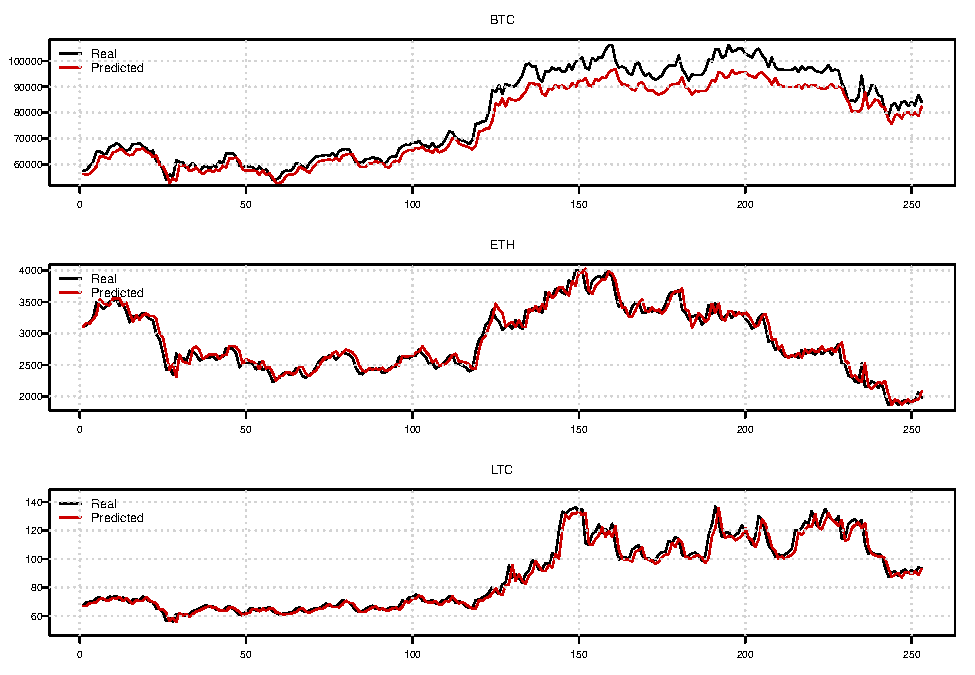
\includegraphics{SoftwareCode_files/figure-latex/unnamed-chunk-18-1.pdf}

\begin{Shaded}
\begin{Highlighting}[]
\DocumentationTok{\#\#\#\#\#\#\#\#\#\#\#\#\#\#\#\#\#\#\#\#\#\#\#\#\#\#\#\#\#\#\#\#\#\#\#\#\#\#\#\#\#\#\#\#\#}

\FunctionTok{par}\NormalTok{(}\AttributeTok{mfrow=}\FunctionTok{c}\NormalTok{(}\DecValTok{3}\NormalTok{,}\DecValTok{1}\NormalTok{), }\AttributeTok{mar=}\FunctionTok{c}\NormalTok{(}\DecValTok{2}\NormalTok{,}\FloatTok{2.5}\NormalTok{,}\DecValTok{2}\NormalTok{,}\DecValTok{1}\NormalTok{), }\AttributeTok{mgp=}\FunctionTok{c}\NormalTok{(}\FloatTok{0.8}\NormalTok{,}\FloatTok{0.35}\NormalTok{,}\DecValTok{0}\NormalTok{), }\AttributeTok{cex.axis=}\FloatTok{0.6}\NormalTok{, }\AttributeTok{tck =} \SpecialCharTok{{-}}\FloatTok{0.05}\NormalTok{)}
\FunctionTok{plot}\NormalTok{(test\_btc, }\AttributeTok{type=}\StringTok{"l"}\NormalTok{, }\AttributeTok{las=}\DecValTok{1}\NormalTok{ , }\AttributeTok{xlab=}\StringTok{""}\NormalTok{, }\AttributeTok{ylab=}\StringTok{""}\NormalTok{ )}
\FunctionTok{lines}\NormalTok{(GRU\_pred\_btc , }\AttributeTok{col=}\StringTok{"red3"}\NormalTok{ )}
\FunctionTok{legend}\NormalTok{(}\StringTok{"topleft"}\NormalTok{, }\AttributeTok{bty=}\StringTok{"n"}\NormalTok{, }\AttributeTok{col=}\FunctionTok{c}\NormalTok{(}\DecValTok{1}\NormalTok{,}\StringTok{"red3"}\NormalTok{), }\AttributeTok{legend=}\FunctionTok{c}\NormalTok{(}\StringTok{"Real"}\NormalTok{, }\StringTok{"Predicted"}\NormalTok{), }\AttributeTok{lty=}\DecValTok{1}\NormalTok{, }\AttributeTok{cex=}\FloatTok{0.7}\NormalTok{ )}
\FunctionTok{grid}\NormalTok{()}
\FunctionTok{title}\NormalTok{(}\StringTok{"BTC"}\NormalTok{, }\AttributeTok{cex.main=}\FloatTok{0.8}\NormalTok{, }\AttributeTok{font.main=}\DecValTok{1}\NormalTok{)}
\DocumentationTok{\#\#\#\#\#\#\#\#\#\#\#\#\#\#\#\#\#\#\#\#\#\#\#\#\#\#\#\#\#\#\#\#\#\#\#\#\#\#\#\#\#\#\#\#\#\#\#\#\#}
\FunctionTok{plot}\NormalTok{(test\_eth, }\AttributeTok{type=}\StringTok{"l"}\NormalTok{, }\AttributeTok{las=}\DecValTok{1}\NormalTok{ , }\AttributeTok{xlab=}\StringTok{""}\NormalTok{, }\AttributeTok{ylab=}\StringTok{""}\NormalTok{ )}
\FunctionTok{lines}\NormalTok{(GRU\_pred\_eth, }\AttributeTok{col=}\StringTok{"red3"}\NormalTok{ )}
\FunctionTok{legend}\NormalTok{(}\StringTok{"topleft"}\NormalTok{, }\AttributeTok{bty=}\StringTok{"n"}\NormalTok{, }\AttributeTok{col=}\FunctionTok{c}\NormalTok{(}\DecValTok{1}\NormalTok{,}\StringTok{"red3"}\NormalTok{), }\AttributeTok{legend=}\FunctionTok{c}\NormalTok{(}\StringTok{"Real"}\NormalTok{, }\StringTok{"Predicted"}\NormalTok{), }\AttributeTok{lty=}\DecValTok{1}\NormalTok{, }\AttributeTok{cex=}\FloatTok{0.7}\NormalTok{ )}
\FunctionTok{grid}\NormalTok{()}
\FunctionTok{title}\NormalTok{(}\StringTok{"ETH"}\NormalTok{, }\AttributeTok{cex.main=}\FloatTok{0.8}\NormalTok{, }\AttributeTok{font.main=}\DecValTok{1}\NormalTok{)}
\DocumentationTok{\#\#\#\#\#\#\#\#\#\#\#\#\#\#\#\#\#\#\#\#\#\#\#\#\#\#\#\#\#\#\#\#\#\#\#\#\#\#\#\#\#\#\#\#\#\#\#\#\#\#\#}
\FunctionTok{plot}\NormalTok{(test\_ltc, }\AttributeTok{type=}\StringTok{"l"}\NormalTok{, }\AttributeTok{las=}\DecValTok{1}\NormalTok{ , }\AttributeTok{xlab=}\StringTok{""}\NormalTok{, }\AttributeTok{ylab=}\StringTok{""}\NormalTok{, }\AttributeTok{ylim=}\FunctionTok{c}\NormalTok{(}\DecValTok{50}\NormalTok{,}\DecValTok{145}\NormalTok{))}
\FunctionTok{lines}\NormalTok{(GRU\_pred\_ltc, }\AttributeTok{col=}\StringTok{"red3"}\NormalTok{ )}
\FunctionTok{legend}\NormalTok{(}\StringTok{"topleft"}\NormalTok{, }\AttributeTok{bty=}\StringTok{"n"}\NormalTok{, }\AttributeTok{col=}\FunctionTok{c}\NormalTok{(}\DecValTok{1}\NormalTok{,}\StringTok{"red3"}\NormalTok{), }\AttributeTok{legend=}\FunctionTok{c}\NormalTok{(}\StringTok{"Real"}\NormalTok{, }\StringTok{"Predicted"}\NormalTok{), }\AttributeTok{lty=}\DecValTok{1}\NormalTok{, }\AttributeTok{cex=}\FloatTok{0.7}\NormalTok{ )}
\FunctionTok{grid}\NormalTok{()}
\FunctionTok{title}\NormalTok{(}\StringTok{"LTC"}\NormalTok{, }\AttributeTok{cex.main=}\FloatTok{0.8}\NormalTok{, }\AttributeTok{font.main=}\DecValTok{1}\NormalTok{)}
\end{Highlighting}
\end{Shaded}

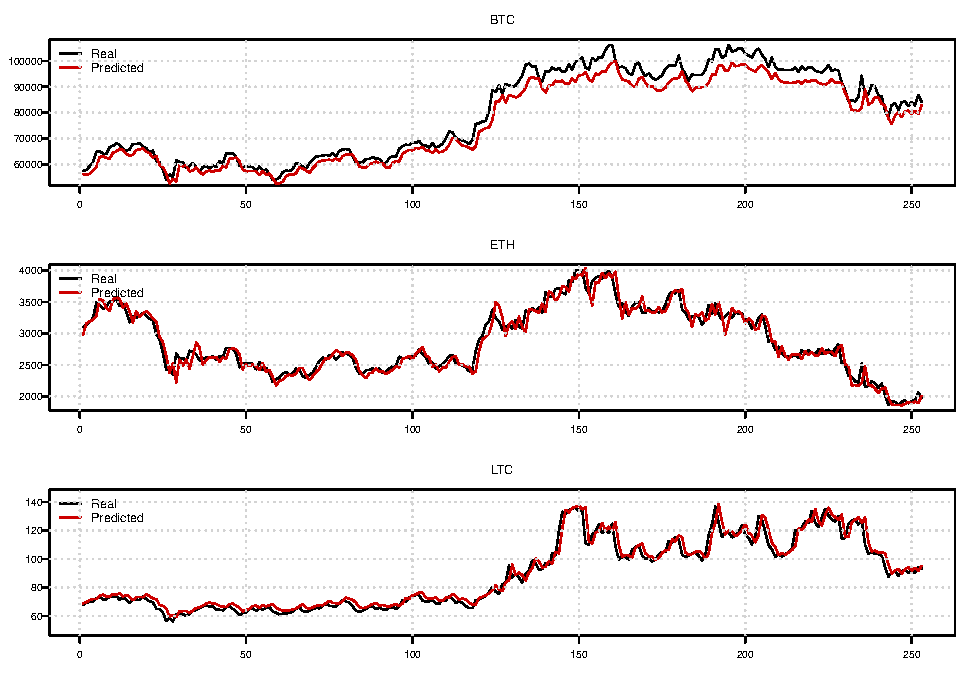
\includegraphics{SoftwareCode_files/figure-latex/unnamed-chunk-18-2.pdf}

\begin{Shaded}
\begin{Highlighting}[]
\DocumentationTok{\#\#\#\#\#\#\#\#\#\#\#\#\#\#\#\#\#\#\#\#\#\#\#\#\#\#\#\#\#\#\#\#\#\#\#\#\#}
\NormalTok{btc\_comb\_tr}\OtherTok{=}\FunctionTok{cbind}\NormalTok{(LSTM\_fit\_btc, GRU\_fit\_btc )}
\NormalTok{btc\_comb\_tst}\OtherTok{=}\FunctionTok{cbind}\NormalTok{(LSTM\_pred\_btc, GRU\_pred\_btc)}
\DocumentationTok{\#\#\#\#\#\#\#\#\#\#\#\#\#\#}
\NormalTok{eth\_comb\_tr}\OtherTok{=}\FunctionTok{cbind}\NormalTok{(LSTM\_fit\_eth, GRU\_fit\_eth )}
\NormalTok{eth\_comb\_tst}\OtherTok{=}\FunctionTok{cbind}\NormalTok{(LSTM\_pred\_eth, GRU\_pred\_eth)}
\DocumentationTok{\#\#\#\#\#\#\#\#\#\#\#\#\#\#\#\#\#\#\#\#\#\#\#\#\#\#\#\#\#\#\#\#\#\#\#\#\#\#\#\#\#\#\#\#\#\#\#\#}
\NormalTok{ltc\_comb\_tr}\OtherTok{=}\FunctionTok{cbind}\NormalTok{(LSTM\_fit\_ltc, GRU\_fit\_ltc )}
\NormalTok{ltc\_comb\_tst}\OtherTok{=}\FunctionTok{cbind}\NormalTok{(LSTM\_pred\_ltc, GRU\_pred\_ltc)}
\FunctionTok{require}\NormalTok{(ForecastComb, }\AttributeTok{quietly=}\NormalTok{T)}
\end{Highlighting}
\end{Shaded}

\begin{verbatim}
## Warning: le package 'ForecastComb' a été compilé avec la version R 4.4.3
\end{verbatim}

\begin{verbatim}
## Registered S3 method overwritten by 'quantmod':
##   method            from
##   as.zoo.data.frame zoo
\end{verbatim}

\begin{Shaded}
\begin{Highlighting}[]
\NormalTok{btc\_df}\OtherTok{=}\FunctionTok{foreccomb}\NormalTok{(train\_btc,btc\_comb\_tr,test\_btc, btc\_comb\_tst)}
\NormalTok{eth\_df}\OtherTok{=}\FunctionTok{foreccomb}\NormalTok{(train\_eth,eth\_comb\_tr,test\_eth, eth\_comb\_tst)}
\NormalTok{ltc\_df}\OtherTok{=}\FunctionTok{foreccomb}\NormalTok{(train\_ltc,ltc\_comb\_tr,test\_ltc, ltc\_comb\_tst)}
\CommentTok{\# OLS}
\NormalTok{ols\_btc}\OtherTok{=}\FunctionTok{comb\_OLS}\NormalTok{(btc\_df)}
\NormalTok{ols\_eth}\OtherTok{=}\FunctionTok{comb\_OLS}\NormalTok{(eth\_df)}
\NormalTok{ols\_ltc}\OtherTok{=}\FunctionTok{comb\_OLS}\NormalTok{(ltc\_df)}
\CommentTok{\# BG}
\NormalTok{bg\_btc}\OtherTok{=}\FunctionTok{comb\_BG}\NormalTok{(btc\_df)}
\NormalTok{bg\_eth}\OtherTok{=}\FunctionTok{comb\_BG}\NormalTok{(eth\_df)}
\NormalTok{bg\_ltc}\OtherTok{=}\FunctionTok{comb\_BG}\NormalTok{(ltc\_df)}
\CommentTok{\# SA}
\NormalTok{sa\_btc}\OtherTok{=}\FunctionTok{comb\_SA}\NormalTok{(btc\_df)}
\NormalTok{sa\_eth}\OtherTok{=}\FunctionTok{comb\_SA}\NormalTok{(eth\_df)}
\NormalTok{sa\_ltc}\OtherTok{=}\FunctionTok{comb\_SA}\NormalTok{(ltc\_df)}

\FunctionTok{options}\NormalTok{(}\AttributeTok{scipen =} \DecValTok{999}\NormalTok{)}
\FunctionTok{par}\NormalTok{(}\AttributeTok{mfrow=}\FunctionTok{c}\NormalTok{(}\DecValTok{3}\NormalTok{,}\DecValTok{1}\NormalTok{), }\AttributeTok{mar=}\FunctionTok{c}\NormalTok{(}\DecValTok{2}\NormalTok{,}\FloatTok{2.5}\NormalTok{,}\DecValTok{2}\NormalTok{,}\DecValTok{1}\NormalTok{), }\AttributeTok{mgp=}\FunctionTok{c}\NormalTok{(}\FloatTok{0.8}\NormalTok{,}\FloatTok{0.35}\NormalTok{,}\DecValTok{0}\NormalTok{), }\AttributeTok{cex.axis=}\FloatTok{0.6}\NormalTok{, }\AttributeTok{tck =} \SpecialCharTok{{-}}\FloatTok{0.05}\NormalTok{)}
\FunctionTok{plot}\NormalTok{(test\_btc, }\AttributeTok{type=}\StringTok{"l"}\NormalTok{, }\AttributeTok{las=}\DecValTok{1}\NormalTok{ , }\AttributeTok{xlab=}\StringTok{""}\NormalTok{, }\AttributeTok{ylab=}\StringTok{""}\NormalTok{ )}
\FunctionTok{lines}\NormalTok{(ols\_btc}\SpecialCharTok{$}\NormalTok{Forecasts\_Test, }\AttributeTok{col=}\StringTok{"red3"}\NormalTok{ )}
\FunctionTok{lines}\NormalTok{(bg\_btc}\SpecialCharTok{$}\NormalTok{Forecasts\_Test, }\AttributeTok{col=}\StringTok{"blue4"}\NormalTok{ )}
\FunctionTok{lines}\NormalTok{(sa\_btc}\SpecialCharTok{$}\NormalTok{Forecasts\_Test, }\AttributeTok{col=}\StringTok{"pink4"}\NormalTok{, }\AttributeTok{lty=}\DecValTok{2}\NormalTok{ )}
\FunctionTok{legend}\NormalTok{(}\StringTok{"topleft"}\NormalTok{, }\AttributeTok{bty=}\StringTok{"n"}\NormalTok{, }\AttributeTok{col=}\FunctionTok{c}\NormalTok{(}\DecValTok{1}\NormalTok{,}\StringTok{"red3"}\NormalTok{, }\StringTok{"blue4"}\NormalTok{, }\StringTok{"pink4"}\NormalTok{), }\AttributeTok{legend=}\FunctionTok{c}\NormalTok{(}\StringTok{"Real"}\NormalTok{, }\StringTok{"OLS"}\NormalTok{, }\StringTok{"BG"}\NormalTok{, }\StringTok{"SA"}\NormalTok{), }\AttributeTok{lty=}\FunctionTok{c}\NormalTok{(}\DecValTok{1}\NormalTok{,}\DecValTok{1}\NormalTok{,}\DecValTok{1}\NormalTok{,}\DecValTok{2}\NormalTok{), }\AttributeTok{cex=}\FloatTok{0.7}\NormalTok{ )}
\FunctionTok{grid}\NormalTok{()}
\FunctionTok{title}\NormalTok{(}\StringTok{"BTC"}\NormalTok{, }\AttributeTok{cex.main=}\FloatTok{0.8}\NormalTok{, }\AttributeTok{font.main=}\DecValTok{1}\NormalTok{)}
\DocumentationTok{\#\#\#\#\#\#\#\#\#\#\#\#\#\#\#\#\#\#\#\#\#\#\#\#\#\#\#\#\#\#\#\#\#\#\#\#\#\#\#\#\#\#\#\#\#\#\#\#\#}
\FunctionTok{plot}\NormalTok{(test\_eth, }\AttributeTok{type=}\StringTok{"l"}\NormalTok{, }\AttributeTok{las=}\DecValTok{1}\NormalTok{ , }\AttributeTok{xlab=}\StringTok{""}\NormalTok{, }\AttributeTok{ylab=}\StringTok{""}\NormalTok{ )}
\FunctionTok{lines}\NormalTok{(ols\_eth}\SpecialCharTok{$}\NormalTok{Forecasts\_Test, }\AttributeTok{col=}\StringTok{"red3"}\NormalTok{ )}
\FunctionTok{lines}\NormalTok{(bg\_eth}\SpecialCharTok{$}\NormalTok{Forecasts\_Test, }\AttributeTok{col=}\StringTok{"blue4"}\NormalTok{ )}
\FunctionTok{lines}\NormalTok{(sa\_eth}\SpecialCharTok{$}\NormalTok{Forecasts\_Test, }\AttributeTok{col=}\StringTok{"pink4"}\NormalTok{, }\AttributeTok{lty=}\DecValTok{2}\NormalTok{ )}
\FunctionTok{legend}\NormalTok{(}\StringTok{"topleft"}\NormalTok{, }\AttributeTok{bty=}\StringTok{"n"}\NormalTok{, }\AttributeTok{col=}\FunctionTok{c}\NormalTok{(}\DecValTok{1}\NormalTok{,}\StringTok{"red3"}\NormalTok{, }\StringTok{"blue4"}\NormalTok{, }\StringTok{"pink4"}\NormalTok{), }\AttributeTok{legend=}\FunctionTok{c}\NormalTok{(}\StringTok{"Real"}\NormalTok{, }\StringTok{"OLS"}\NormalTok{, }\StringTok{"BG"}\NormalTok{, }\StringTok{"SA"}\NormalTok{), }\AttributeTok{lty=}\FunctionTok{c}\NormalTok{(}\DecValTok{1}\NormalTok{,}\DecValTok{1}\NormalTok{,}\DecValTok{1}\NormalTok{,}\DecValTok{2}\NormalTok{), }\AttributeTok{cex=}\FloatTok{0.7}\NormalTok{ )}
\FunctionTok{grid}\NormalTok{()}
\FunctionTok{title}\NormalTok{(}\StringTok{"ETH"}\NormalTok{, }\AttributeTok{cex.main=}\FloatTok{0.8}\NormalTok{, }\AttributeTok{font.main=}\DecValTok{1}\NormalTok{)}
\DocumentationTok{\#\#\#\#\#\#\#\#\#\#\#\#\#\#\#\#\#\#\#\#\#\#\#\#\#\#\#\#\#\#\#\#\#\#\#\#\#\#\#\#\#\#\#\#\#\#\#\#\#\#\#}
\FunctionTok{plot}\NormalTok{(test\_ltc, }\AttributeTok{type=}\StringTok{"l"}\NormalTok{, }\AttributeTok{las=}\DecValTok{1}\NormalTok{ , }\AttributeTok{xlab=}\StringTok{""}\NormalTok{, }\AttributeTok{ylab=}\StringTok{""}\NormalTok{, }\AttributeTok{ylim=}\FunctionTok{c}\NormalTok{(}\DecValTok{50}\NormalTok{,}\DecValTok{145}\NormalTok{) )}
\FunctionTok{lines}\NormalTok{(ols\_ltc}\SpecialCharTok{$}\NormalTok{Forecasts\_Test, }\AttributeTok{col=}\StringTok{"red3"}\NormalTok{ )}
\FunctionTok{lines}\NormalTok{(bg\_ltc}\SpecialCharTok{$}\NormalTok{Forecasts\_Test, }\AttributeTok{col=}\StringTok{"blue4"}\NormalTok{ )}
\FunctionTok{lines}\NormalTok{(sa\_ltc}\SpecialCharTok{$}\NormalTok{Forecasts\_Test, }\AttributeTok{col=}\StringTok{"pink4"}\NormalTok{, }\AttributeTok{lty=}\DecValTok{2}\NormalTok{ )}
\FunctionTok{legend}\NormalTok{(}\StringTok{"topleft"}\NormalTok{, }\AttributeTok{bty=}\StringTok{"n"}\NormalTok{, }\AttributeTok{col=}\FunctionTok{c}\NormalTok{(}\DecValTok{1}\NormalTok{,}\StringTok{"red3"}\NormalTok{, }\StringTok{"blue4"}\NormalTok{, }\StringTok{"pink4"}\NormalTok{), }\AttributeTok{legend=}\FunctionTok{c}\NormalTok{(}\StringTok{"Real"}\NormalTok{, }\StringTok{"OLS"}\NormalTok{, }\StringTok{"BG"}\NormalTok{, }\StringTok{"SA"}\NormalTok{), }\AttributeTok{lty=}\FunctionTok{c}\NormalTok{(}\DecValTok{1}\NormalTok{,}\DecValTok{1}\NormalTok{,}\DecValTok{1}\NormalTok{,}\DecValTok{2}\NormalTok{), }\AttributeTok{cex=}\FloatTok{0.7}\NormalTok{ )}
\FunctionTok{grid}\NormalTok{()}
\FunctionTok{title}\NormalTok{(}\StringTok{"LTC"}\NormalTok{, }\AttributeTok{cex.main=}\FloatTok{0.8}\NormalTok{, }\AttributeTok{font.main=}\DecValTok{1}\NormalTok{)}
\end{Highlighting}
\end{Shaded}

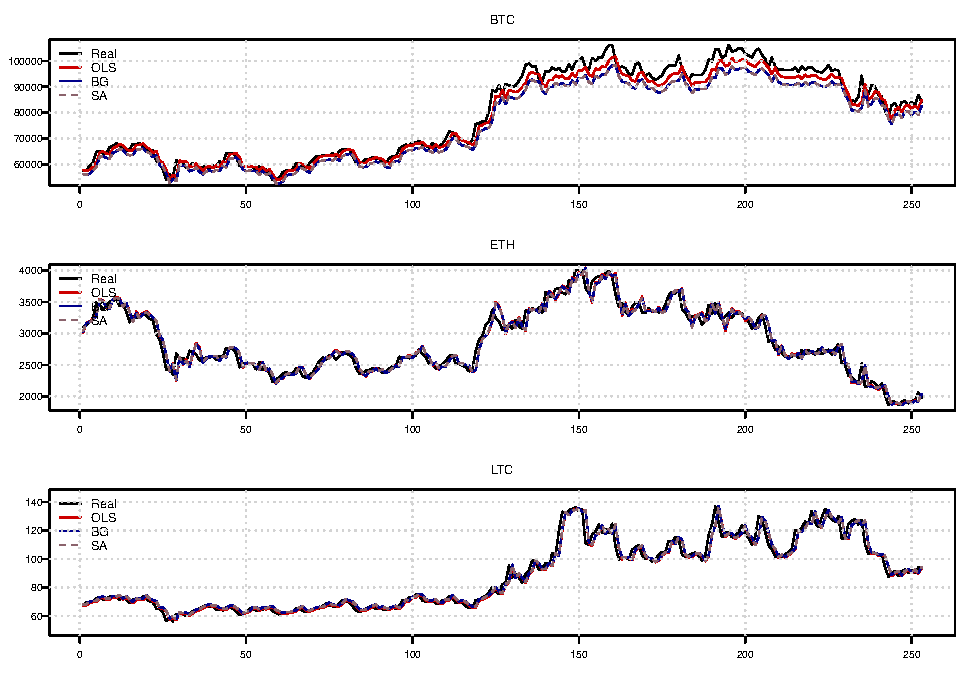
\includegraphics{SoftwareCode_files/figure-latex/unnamed-chunk-18-3.pdf}

\begin{Shaded}
\begin{Highlighting}[]
\NormalTok{metriks}\OtherTok{=}\ControlFlowTok{function}\NormalTok{(x,y)\{}
  \FunctionTok{require}\NormalTok{(Metrics, }\AttributeTok{quietly =}\NormalTok{ T)}
\NormalTok{  rr}\OtherTok{=}\FunctionTok{c}\NormalTok{(}\AttributeTok{RMSE=}\FunctionTok{rmse}\NormalTok{(x,y), }\AttributeTok{RMAE=}\FunctionTok{mae}\NormalTok{(x,y)}\SpecialCharTok{**}\FloatTok{0.5}\NormalTok{, }\AttributeTok{MAPE=}\FunctionTok{mape}\NormalTok{(x,y)}\SpecialCharTok{*}\DecValTok{100}\NormalTok{)}
\NormalTok{  rr}
\NormalTok{  \}}
\end{Highlighting}
\end{Shaded}

\begin{Shaded}
\begin{Highlighting}[]
\NormalTok{acc\_btc\_lstm}\OtherTok{=}\FunctionTok{c}\NormalTok{(}\FunctionTok{metriks}\NormalTok{(train\_btc,LSTM\_fit\_btc),}\FunctionTok{metriks}\NormalTok{(test\_btc,LSTM\_pred\_btc))}
\NormalTok{acc\_btc\_gru}\OtherTok{=}\FunctionTok{c}\NormalTok{(}\FunctionTok{metriks}\NormalTok{(train\_btc,GRU\_fit\_btc),}\FunctionTok{metriks}\NormalTok{(test\_btc,GRU\_pred\_btc))}
\NormalTok{acc\_btc\_ols}\OtherTok{=}\FunctionTok{c}\NormalTok{(}\FunctionTok{metriks}\NormalTok{(train\_btc,ols\_btc}\SpecialCharTok{$}\NormalTok{Fitted),}\FunctionTok{metriks}\NormalTok{(test\_btc,ols\_btc}\SpecialCharTok{$}\NormalTok{Forecasts\_Test))}
\NormalTok{acc\_btc\_bg}\OtherTok{=}\FunctionTok{c}\NormalTok{(}\FunctionTok{metriks}\NormalTok{(train\_btc,bg\_btc}\SpecialCharTok{$}\NormalTok{Fitted),}\FunctionTok{metriks}\NormalTok{(test\_btc,bg\_btc}\SpecialCharTok{$}\NormalTok{Forecasts\_Test))}
\NormalTok{acc\_btc\_sa}\OtherTok{=}\FunctionTok{c}\NormalTok{(}\FunctionTok{metriks}\NormalTok{(train\_btc,sa\_btc}\SpecialCharTok{$}\NormalTok{Fitted),}\FunctionTok{metriks}\NormalTok{(test\_btc,sa\_btc}\SpecialCharTok{$}\NormalTok{Forecasts\_Test))}
\NormalTok{t1}\OtherTok{=}\FunctionTok{rbind}\NormalTok{(acc\_btc\_lstm, acc\_btc\_gru, acc\_btc\_ols, acc\_btc\_bg, acc\_btc\_sa)}
\end{Highlighting}
\end{Shaded}

\begin{Shaded}
\begin{Highlighting}[]
\NormalTok{acc\_eth\_lstm}\OtherTok{=}\FunctionTok{c}\NormalTok{(}\FunctionTok{metriks}\NormalTok{(train\_eth,LSTM\_fit\_eth),}\FunctionTok{metriks}\NormalTok{(test\_eth,LSTM\_pred\_eth))}
\NormalTok{acc\_eth\_gru}\OtherTok{=}\FunctionTok{c}\NormalTok{(}\FunctionTok{metriks}\NormalTok{(train\_eth,GRU\_fit\_eth),}\FunctionTok{metriks}\NormalTok{(test\_eth,GRU\_pred\_eth))}
\NormalTok{acc\_eth\_ols}\OtherTok{=}\FunctionTok{c}\NormalTok{(}\FunctionTok{metriks}\NormalTok{(train\_eth,ols\_eth}\SpecialCharTok{$}\NormalTok{Fitted),}\FunctionTok{metriks}\NormalTok{(test\_eth,ols\_eth}\SpecialCharTok{$}\NormalTok{Forecasts\_Test))}
\NormalTok{acc\_eth\_bg}\OtherTok{=}\FunctionTok{c}\NormalTok{(}\FunctionTok{metriks}\NormalTok{(train\_eth,bg\_eth}\SpecialCharTok{$}\NormalTok{Fitted),}\FunctionTok{metriks}\NormalTok{(test\_eth,bg\_eth}\SpecialCharTok{$}\NormalTok{Forecasts\_Test))}
\NormalTok{acc\_eth\_sa}\OtherTok{=}\FunctionTok{c}\NormalTok{(}\FunctionTok{metriks}\NormalTok{(train\_eth,sa\_eth}\SpecialCharTok{$}\NormalTok{Fitted),}\FunctionTok{metriks}\NormalTok{(test\_eth,sa\_eth}\SpecialCharTok{$}\NormalTok{Forecasts\_Test))}
\NormalTok{t2}\OtherTok{=}\FunctionTok{rbind}\NormalTok{(acc\_eth\_lstm, acc\_eth\_gru, acc\_eth\_ols, acc\_eth\_bg, acc\_eth\_sa)}
\end{Highlighting}
\end{Shaded}

\begin{Shaded}
\begin{Highlighting}[]
\NormalTok{acc\_ltc\_lstm}\OtherTok{=}\FunctionTok{c}\NormalTok{(}\FunctionTok{metriks}\NormalTok{(train\_ltc,LSTM\_fit\_ltc),}\FunctionTok{metriks}\NormalTok{(test\_ltc,LSTM\_pred\_ltc))}
\NormalTok{acc\_ltc\_gru}\OtherTok{=}\FunctionTok{c}\NormalTok{(}\FunctionTok{metriks}\NormalTok{(train\_ltc,GRU\_fit\_ltc),}\FunctionTok{metriks}\NormalTok{(test\_ltc,GRU\_pred\_ltc))}
\NormalTok{acc\_ltc\_ols}\OtherTok{=}\FunctionTok{c}\NormalTok{(}\FunctionTok{metriks}\NormalTok{(train\_ltc,ols\_ltc}\SpecialCharTok{$}\NormalTok{Fitted),}\FunctionTok{metriks}\NormalTok{(test\_ltc,ols\_ltc}\SpecialCharTok{$}\NormalTok{Forecasts\_Test))}
\NormalTok{acc\_ltc\_bg}\OtherTok{=}\FunctionTok{c}\NormalTok{(}\FunctionTok{metriks}\NormalTok{(train\_ltc,bg\_ltc}\SpecialCharTok{$}\NormalTok{Fitted),}\FunctionTok{metriks}\NormalTok{(test\_ltc,bg\_ltc}\SpecialCharTok{$}\NormalTok{Forecasts\_Test))}
\NormalTok{acc\_ltc\_sa}\OtherTok{=}\FunctionTok{c}\NormalTok{(}\FunctionTok{metriks}\NormalTok{(train\_ltc,sa\_ltc}\SpecialCharTok{$}\NormalTok{Fitted),}\FunctionTok{metriks}\NormalTok{(test\_ltc,sa\_ltc}\SpecialCharTok{$}\NormalTok{Forecasts\_Test))}
\NormalTok{t3}\OtherTok{=}\FunctionTok{rbind}\NormalTok{(acc\_ltc\_lstm, acc\_ltc\_gru, acc\_ltc\_ols, acc\_ltc\_bg, acc\_ltc\_sa)}
\end{Highlighting}
\end{Shaded}

\begin{Shaded}
\begin{Highlighting}[]
\NormalTok{cn}\OtherTok{=}\FunctionTok{c}\NormalTok{(}\StringTok{"LSTM"}\NormalTok{, }\StringTok{"GRU"}\NormalTok{, }\StringTok{"Comb\_OLS"}\NormalTok{, }\StringTok{"Comb\_BG"}\NormalTok{, }\StringTok{"Comb\_SA"}\NormalTok{)}
\FunctionTok{row.names}\NormalTok{(t1)}\OtherTok{=}\FunctionTok{row.names}\NormalTok{(t2)}\OtherTok{=}\FunctionTok{row.names}\NormalTok{(t3)}\OtherTok{=}\ConstantTok{NULL}
\NormalTok{rn}\OtherTok{=}\FunctionTok{rep}\NormalTok{(cn,}\DecValTok{3}\NormalTok{)}
\NormalTok{tab}\OtherTok{=}\FunctionTok{data.frame}\NormalTok{(}\FunctionTok{cbind}\NormalTok{(rn,}\FunctionTok{round}\NormalTok{(}\FunctionTok{rbind}\NormalTok{(t1,t2,t3),}\DecValTok{3}\NormalTok{)))}
\FunctionTok{require}\NormalTok{(dplyr, }\AttributeTok{quietly =}\NormalTok{ T)}
\end{Highlighting}
\end{Shaded}

\begin{verbatim}
## 
## Attachement du package : 'dplyr'
\end{verbatim}

\begin{verbatim}
## Les objets suivants sont masqués depuis 'package:stats':
## 
##     filter, lag
\end{verbatim}

\begin{verbatim}
## Les objets suivants sont masqués depuis 'package:base':
## 
##     intersect, setdiff, setequal, union
\end{verbatim}

\begin{Shaded}
\begin{Highlighting}[]
\FunctionTok{require}\NormalTok{(kableExtra, }\AttributeTok{quietly =}\NormalTok{ T)}
\end{Highlighting}
\end{Shaded}

\begin{verbatim}
## Warning: le package 'kableExtra' a été compilé avec la version R 4.4.3
\end{verbatim}

\begin{verbatim}
## 
## Attachement du package : 'kableExtra'
\end{verbatim}

\begin{verbatim}
## L'objet suivant est masqué depuis 'package:dplyr':
## 
##     group_rows
\end{verbatim}

\begin{Shaded}
\begin{Highlighting}[]
\FunctionTok{colnames}\NormalTok{(tab)[}\DecValTok{1}\NormalTok{]}\OtherTok{=}\StringTok{""}
\FunctionTok{kbl}\NormalTok{(tab, }\AttributeTok{digits=}\DecValTok{2}\NormalTok{, }\AttributeTok{align=}\StringTok{"c"}\NormalTok{, }\AttributeTok{booktabs =}\NormalTok{ T) }\SpecialCharTok{\%\textgreater{}\%}
  \FunctionTok{pack\_rows}\NormalTok{(}\StringTok{"BTC"}\NormalTok{, }\DecValTok{1}\NormalTok{, }\DecValTok{5}\NormalTok{) }\SpecialCharTok{\%\textgreater{}\%}
  \FunctionTok{pack\_rows}\NormalTok{(}\StringTok{"ETH"}\NormalTok{, }\DecValTok{6}\NormalTok{, }\DecValTok{10}\NormalTok{) }\SpecialCharTok{\%\textgreater{}\%}
  \FunctionTok{pack\_rows}\NormalTok{(}\StringTok{"LTC"}\NormalTok{, }\DecValTok{11}\NormalTok{, }\DecValTok{15}\NormalTok{) }\SpecialCharTok{\%\textgreater{}\%}
  \FunctionTok{add\_header\_above}\NormalTok{(}\FunctionTok{c}\NormalTok{(}\StringTok{" "} \OtherTok{=} \DecValTok{1}\NormalTok{, }\StringTok{"Train"} \OtherTok{=} \DecValTok{3}\NormalTok{, }\StringTok{"Test"} \OtherTok{=} \DecValTok{3}\NormalTok{))}
\end{Highlighting}
\end{Shaded}

\begin{tabular}[t]{ccccccc}
\toprule
\multicolumn{1}{c}{ } & \multicolumn{3}{c}{Train} & \multicolumn{3}{c}{Test} \\
\cmidrule(l{3pt}r{3pt}){2-4} \cmidrule(l{3pt}r{3pt}){5-7}
 & RMSE & RMAE & MAPE & RMSE.1 & RMAE.1 & MAPE.1\\
\midrule
\addlinespace[0.3em]
\multicolumn{7}{l}{\textbf{BTC}}\\
\hspace{1em}LSTM & 1390.264 & 31.308 & 4.563 & 5358.839 & 66.428 & 5.114\\
\hspace{1em}GRU & 1308.704 & 28.497 & 3.073 & 4311.471 & 59.87 & 4.282\\
\hspace{1em}Comb\_OLS & 1033.683 & 24.165 & 2.396 & 2987.408 & 47.695 & 2.693\\
\hspace{1em}Comb\_BG & 1340.918 & 29.712 & 3.662 & 4786.434 & 63.029 & 4.672\\
\hspace{1em}Comb\_SA & 1343.37 & 29.799 & 3.709 & 4818.105 & 63.227 & 4.697\\
\addlinespace[0.3em]
\multicolumn{7}{l}{\textbf{ETH}}\\
\hspace{1em}LSTM & 74.317 & 7.253 & 8.811 & 114.527 & 9.216 & 2.99\\
\hspace{1em}GRU & 62.238 & 6.376 & 4.426 & 125.011 & 9.693 & 3.264\\
\hspace{1em}Comb\_OLS & 59.769 & 6.114 & 4.288 & 120.632 & 9.469 & 3.115\\
\hspace{1em}Comb\_BG & 62.258 & 6.478 & 5.764 & 117.045 & 9.313 & 3.018\\
\hspace{1em}Comb\_SA & 63.24 & 6.556 & 6.15 & 115.978 & 9.262 & 2.987\\
\addlinespace[0.3em]
\multicolumn{7}{l}{\textbf{LTC}}\\
\hspace{1em}LSTM & 6.586 & 1.948 & 3.781 & 4.845 & 1.792 & 3.341\\
\hspace{1em}GRU & 6.118 & 2.02 & 4.749 & 4.977 & 1.856 & 3.81\\
\hspace{1em}Comb\_OLS & 5.801 & 1.845 & 3.424 & 4.728 & 1.755 & 3.214\\
\hspace{1em}Comb\_BG & 5.974 & 1.914 & 3.981 & 4.698 & 1.758 & 3.261\\
\hspace{1em}Comb\_SA & 5.99 & 1.91 & 3.941 & 4.691 & 1.755 & 3.244\\
\bottomrule
\end{tabular}

\begin{Shaded}
\begin{Highlighting}[]
\FunctionTok{require}\NormalTok{(dplyr, }\AttributeTok{quietly =}\NormalTok{ T)}
\FunctionTok{require}\NormalTok{(kableExtra, }\AttributeTok{quietly =}\NormalTok{ T)}
\NormalTok{collapse\_rows\_dt }\OtherTok{\textless{}{-}} \FunctionTok{data.frame}\NormalTok{(}\AttributeTok{C1 =} \FunctionTok{c}\NormalTok{(}\FunctionTok{rep}\NormalTok{(}\StringTok{"a"}\NormalTok{, }\DecValTok{10}\NormalTok{), }\FunctionTok{rep}\NormalTok{(}\StringTok{"b"}\NormalTok{, }\DecValTok{5}\NormalTok{)),}
\AttributeTok{C2 =} \FunctionTok{c}\NormalTok{(}\FunctionTok{rep}\NormalTok{(}\StringTok{"c"}\NormalTok{, }\DecValTok{7}\NormalTok{), }\FunctionTok{rep}\NormalTok{(}\StringTok{"d"}\NormalTok{, }\DecValTok{3}\NormalTok{), }\FunctionTok{rep}\NormalTok{(}\StringTok{"c"}\NormalTok{, }\DecValTok{2}\NormalTok{), }\FunctionTok{rep}\NormalTok{(}\StringTok{"d"}\NormalTok{, }\DecValTok{3}\NormalTok{)),}
\AttributeTok{C3 =} \DecValTok{1}\SpecialCharTok{:}\DecValTok{15}\NormalTok{,}
\AttributeTok{C4 =} \FunctionTok{sample}\NormalTok{(}\FunctionTok{c}\NormalTok{(}\DecValTok{0}\NormalTok{,}\DecValTok{1}\NormalTok{), }\DecValTok{15}\NormalTok{, }\AttributeTok{replace =} \ConstantTok{TRUE}\NormalTok{))}
\FunctionTok{kbl}\NormalTok{(collapse\_rows\_dt[}\SpecialCharTok{{-}}\DecValTok{1}\NormalTok{], }\AttributeTok{align =} \StringTok{"c"}\NormalTok{, }\AttributeTok{booktabs =}\NormalTok{ T) }\SpecialCharTok{\%\textgreater{}\%}
\FunctionTok{column\_spec}\NormalTok{(}\DecValTok{1}\NormalTok{, }\AttributeTok{bold =}\NormalTok{ T, }\AttributeTok{width =} \StringTok{"5em"}\NormalTok{) }\SpecialCharTok{\%\textgreater{}\%}
\FunctionTok{row\_spec}\NormalTok{(}\FunctionTok{c}\NormalTok{(}\DecValTok{1}\SpecialCharTok{:}\DecValTok{7}\NormalTok{, }\DecValTok{11}\SpecialCharTok{:}\DecValTok{12}\NormalTok{) }\SpecialCharTok{{-}} \DecValTok{1}\NormalTok{, }\AttributeTok{extra\_latex\_after =} \StringTok{"}\SpecialCharTok{\textbackslash{}\textbackslash{}}\StringTok{rowcolor\{gray!6\}"}\NormalTok{) }\SpecialCharTok{\%\textgreater{}\%}
\FunctionTok{collapse\_rows}\NormalTok{(}\DecValTok{1}\NormalTok{, }\AttributeTok{latex\_hline =} \StringTok{"none"}\NormalTok{)}
\end{Highlighting}
\end{Shaded}


\end{document}
